% v1: three explanatory concepts; schematic signals, no inferred latent geometry.
\documentclass[tikz,border=0pt]{standalone}
\usepackage{amsmath}
\usetikzlibrary{arrows.meta,calc}
\definecolor{hl}{HTML}{0092B5}
\tikzset{>=Latex,line width=.7pt, lab/.style={font=\small},
 fixed/.style={black!55},learn/.style={hl},
 blk/.style={draw,rounded corners=1pt,minimum width=13mm,minimum height=7mm}}
\begin{document}
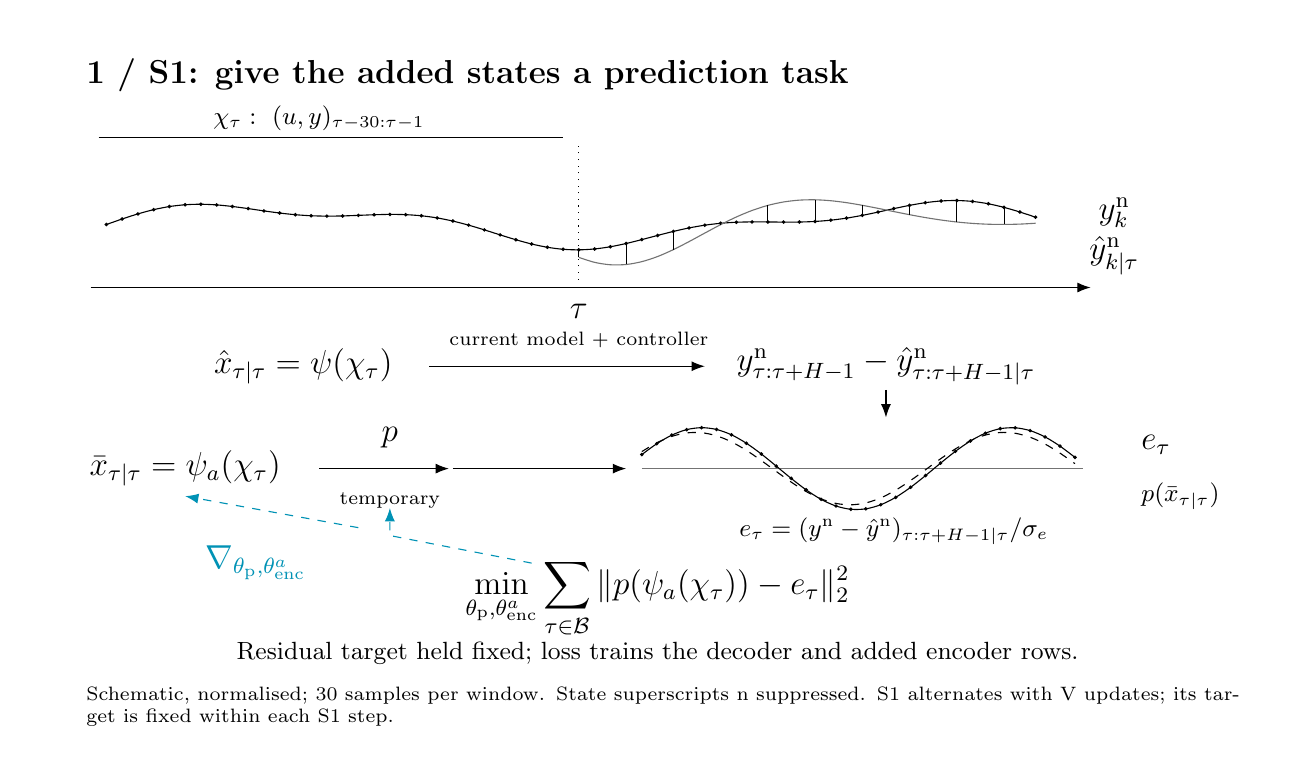
\begin{tikzpicture}\useasboundingbox (0,0) rectangle (16,9);\fill[white] (0,0) rectangle (16,9);\fontsize{12}{14}\selectfont
\node[anchor=west,font=\large\bfseries] at (0.6,8.4) {1 / S1: give the added states a prediction task};
\node[anchor=west,font=\scriptsize,text width=14.8cm,align=left] at (0.6,0.38) {Schematic, normalised; 30 samples per window. State superscripts n suppressed. S1 alternates with V updates; its target is fixed within each S1 step.};
\draw[black] plot[smooth] coordinates {(1.0000,6.5000) (1.2000,6.5703) (1.4000,6.6348) (1.6000,6.6887) (1.8000,6.7281) (2.0000,6.7510) (2.2000,6.7574) (2.4000,6.7490) (2.6000,6.7291) (2.8000,6.7022) (3.0000,6.6730) (3.2000,6.6459) (3.4000,6.6246) (3.6000,6.6113) (3.8000,6.6065) (4.0000,6.6091) (4.2000,6.6162) (4.4000,6.6241) (4.6000,6.6285) (4.8000,6.6252) (5.0000,6.6110) (5.2000,6.5839) (5.4000,6.5437) (5.6000,6.4919) (5.8000,6.4319) (6.0000,6.3684) (6.2000,6.3068) (6.4000,6.2527) (6.6000,6.2110) (6.8000,6.1855) (7.0000,6.1784) (7.2000,6.1897) (7.4000,6.2177) (7.6000,6.2588) (7.8000,6.3085) (8.0000,6.3614) (8.2000,6.4122) (8.4000,6.4567) (8.6000,6.4916) (8.8000,6.5155) (9.0000,6.5287) (9.2000,6.5334) (9.4000,6.5326) (9.6000,6.5306) (9.8000,6.5315) (10.0000,6.5389) (10.2000,6.5551) (10.4000,6.5812) (10.6000,6.6163) (10.8000,6.6577) (11.0000,6.7017) (11.2000,6.7432) (11.4000,6.7772) (11.6000,6.7990) (11.8000,6.8050) (12.0000,6.7932) (12.2000,6.7635) (12.4000,6.7175) (12.6000,6.6591) (12.8000,6.5929)};
\fill[black] (1.0000,6.5000) circle (.025);
\fill[black] (1.2000,6.5703) circle (.025);
\fill[black] (1.4000,6.6348) circle (.025);
\fill[black] (1.6000,6.6887) circle (.025);
\fill[black] (1.8000,6.7281) circle (.025);
\fill[black] (2.0000,6.7510) circle (.025);
\fill[black] (2.2000,6.7574) circle (.025);
\fill[black] (2.4000,6.7490) circle (.025);
\fill[black] (2.6000,6.7291) circle (.025);
\fill[black] (2.8000,6.7022) circle (.025);
\fill[black] (3.0000,6.6730) circle (.025);
\fill[black] (3.2000,6.6459) circle (.025);
\fill[black] (3.4000,6.6246) circle (.025);
\fill[black] (3.6000,6.6113) circle (.025);
\fill[black] (3.8000,6.6065) circle (.025);
\fill[black] (4.0000,6.6091) circle (.025);
\fill[black] (4.2000,6.6162) circle (.025);
\fill[black] (4.4000,6.6241) circle (.025);
\fill[black] (4.6000,6.6285) circle (.025);
\fill[black] (4.8000,6.6252) circle (.025);
\fill[black] (5.0000,6.6110) circle (.025);
\fill[black] (5.2000,6.5839) circle (.025);
\fill[black] (5.4000,6.5437) circle (.025);
\fill[black] (5.6000,6.4919) circle (.025);
\fill[black] (5.8000,6.4319) circle (.025);
\fill[black] (6.0000,6.3684) circle (.025);
\fill[black] (6.2000,6.3068) circle (.025);
\fill[black] (6.4000,6.2527) circle (.025);
\fill[black] (6.6000,6.2110) circle (.025);
\fill[black] (6.8000,6.1855) circle (.025);
\fill[black] (7.0000,6.1784) circle (.025);
\fill[black] (7.2000,6.1897) circle (.025);
\fill[black] (7.4000,6.2177) circle (.025);
\fill[black] (7.6000,6.2588) circle (.025);
\fill[black] (7.8000,6.3085) circle (.025);
\fill[black] (8.0000,6.3614) circle (.025);
\fill[black] (8.2000,6.4122) circle (.025);
\fill[black] (8.4000,6.4567) circle (.025);
\fill[black] (8.6000,6.4916) circle (.025);
\fill[black] (8.8000,6.5155) circle (.025);
\fill[black] (9.0000,6.5287) circle (.025);
\fill[black] (9.2000,6.5334) circle (.025);
\fill[black] (9.4000,6.5326) circle (.025);
\fill[black] (9.6000,6.5306) circle (.025);
\fill[black] (9.8000,6.5315) circle (.025);
\fill[black] (10.0000,6.5389) circle (.025);
\fill[black] (10.2000,6.5551) circle (.025);
\fill[black] (10.4000,6.5812) circle (.025);
\fill[black] (10.6000,6.6163) circle (.025);
\fill[black] (10.8000,6.6577) circle (.025);
\fill[black] (11.0000,6.7017) circle (.025);
\fill[black] (11.2000,6.7432) circle (.025);
\fill[black] (11.4000,6.7772) circle (.025);
\fill[black] (11.6000,6.7990) circle (.025);
\fill[black] (11.8000,6.8050) circle (.025);
\fill[black] (12.0000,6.7932) circle (.025);
\fill[black] (12.2000,6.7635) circle (.025);
\fill[black] (12.4000,6.7175) circle (.025);
\fill[black] (12.6000,6.6591) circle (.025);
\fill[black] (12.8000,6.5929) circle (.025);
\draw[->] (0.8,5.7) -- (13.5,5.7);
\draw[dotted] (7,5.8) -- (7,7.5);
\node[] at (7,5.4) {$\tau$};
\node[] at (13.8,6.65) {$y^{\rm n}_k$};
\draw[] (0.9,7.6) -- (6.8,7.6);
\node[font=\small] at (3.7,7.85) {$\chi_\tau:\ (u,y)_{\tau-30:\tau-1}$};
\draw[black!55] plot[smooth] coordinates {(7.0000,6.0824) (7.2000,6.0195) (7.4000,5.9888) (7.6000,5.9923) (7.8000,6.0285) (8.0000,6.0935) (8.2000,6.1810) (8.4000,6.2832) (8.6000,6.3916) (8.8000,6.4982) (9.0000,6.5957) (9.2000,6.6785) (9.4000,6.7427) (9.6000,6.7864) (9.8000,6.8096) (10.0000,6.8140) (10.2000,6.8021) (10.4000,6.7775) (10.6000,6.7439) (10.8000,6.7051) (11.0000,6.6645) (11.2000,6.6248) (11.4000,6.5884) (11.6000,6.5571) (11.8000,6.5320) (12.0000,6.5141) (12.2000,6.5037) (12.4000,6.5009) (12.6000,6.5052) (12.8000,6.5160)};
\node[black] at (13.8,6.1) {$\hat y^{\rm n}_{k|\tau}$};
\node[black] at (3.5,4.7) {$\hat x_{\tau|\tau}=\psi(\chi_\tau)$};
\draw[black,->] (5.1,4.7) -- (8.6,4.7);
\node[font=\scriptsize,black] at (7,5.03) {current model + controller};
\node[black] at (10.9,4.7) {$y^{\rm n}_{\tau:\tau+H-1}-\hat y^{\rm n}_{\tau:\tau+H-1|\tau}$};
\draw[black] (7.0,6.1784) -- (7.0,6.0824);
\draw[black] (7.6,6.2588) -- (7.6,5.9923);
\draw[black] (8.2,6.4122) -- (8.2,6.181);
\draw[black] (8.8,6.5155) -- (8.8,6.4982);
\draw[black] (9.4,6.5326) -- (9.4,6.7427);
\draw[black] (10.0,6.5389) -- (10.0,6.814);
\draw[black] (10.6,6.6163) -- (10.6,6.7439);
\draw[black] (11.2,6.7432) -- (11.2,6.6248);
\draw[black] (11.8,6.805) -- (11.8,6.532);
\draw[black] (12.4,6.7175) -- (12.4,6.5009);
\draw[black!55] (7.8,3.4) -- (13.4,3.4);
\draw[black] plot[smooth] coordinates {(7.8000,3.5783) (7.9897,3.7161) (8.1793,3.8250) (8.3690,3.8951) (8.5586,3.9200) (8.7483,3.8974) (8.9379,3.8294) (9.1276,3.7222) (9.3172,3.5856) (9.5069,3.4320) (9.6966,3.2756) (9.8862,3.1304) (10.0759,3.0099) (10.2655,2.9250) (10.4552,2.8835) (10.6448,2.8891) (10.8345,2.9414) (11.0241,3.0355) (11.2138,3.1630) (11.4034,3.3120) (11.5931,3.4691) (11.7828,3.6199) (11.9724,3.7506) (12.1621,3.8493) (12.3517,3.9070) (12.5414,3.9184) (12.7310,3.8824) (12.9207,3.8024) (13.1103,3.6857) (13.3000,3.5429)};
\fill[black] (7.8000,3.5783) circle (.025);
\fill[black] (7.9897,3.7161) circle (.025);
\fill[black] (8.1793,3.8250) circle (.025);
\fill[black] (8.3690,3.8951) circle (.025);
\fill[black] (8.5586,3.9200) circle (.025);
\fill[black] (8.7483,3.8974) circle (.025);
\fill[black] (8.9379,3.8294) circle (.025);
\fill[black] (9.1276,3.7222) circle (.025);
\fill[black] (9.3172,3.5856) circle (.025);
\fill[black] (9.5069,3.4320) circle (.025);
\fill[black] (9.6966,3.2756) circle (.025);
\fill[black] (9.8862,3.1304) circle (.025);
\fill[black] (10.0759,3.0099) circle (.025);
\fill[black] (10.2655,2.9250) circle (.025);
\fill[black] (10.4552,2.8835) circle (.025);
\fill[black] (10.6448,2.8891) circle (.025);
\fill[black] (10.8345,2.9414) circle (.025);
\fill[black] (11.0241,3.0355) circle (.025);
\fill[black] (11.2138,3.1630) circle (.025);
\fill[black] (11.4034,3.3120) circle (.025);
\fill[black] (11.5931,3.4691) circle (.025);
\fill[black] (11.7828,3.6199) circle (.025);
\fill[black] (11.9724,3.7506) circle (.025);
\fill[black] (12.1621,3.8493) circle (.025);
\fill[black] (12.3517,3.9070) circle (.025);
\fill[black] (12.5414,3.9184) circle (.025);
\fill[black] (12.7310,3.8824) circle (.025);
\fill[black] (12.9207,3.8024) circle (.025);
\fill[black] (13.1103,3.6857) circle (.025);
\fill[black] (13.3000,3.5429) circle (.025);
\node[anchor=west,black] at (14,3.7) {$e_\tau$};
\draw[->,black] (10.9,4.4) -- (10.9,4.05);
\node[black,font=\small] at (11,2.6) {$e_\tau=(y^{\rm n}-\hat y^{\rm n})_{\tau:\tau+H-1|\tau}/\sigma_e$};
\node[black] at (2,3.4) {$\bar x_{\tau|\tau}=\psi_a(\chi_\tau)$};
\draw[->,black] (3.7,3.4) -- (5.35,3.4);
\node[font=\large,black] at (4.6,3.8) {$p$};
\node[font=\scriptsize,black] at (4.6,3) {temporary};
\draw[black,dashed] plot[smooth] coordinates {(7.8000,3.6165) (7.9897,3.7278) (8.1793,3.8093) (8.3690,3.8533) (8.5586,3.8560) (8.7483,3.8170) (8.9379,3.7400) (9.1276,3.6319) (9.3172,3.5026) (9.5069,3.3640) (9.6966,3.2287) (9.8862,3.1090) (10.0759,3.0159) (10.2655,2.9578) (10.4552,2.9401) (10.6448,2.9644) (10.8345,3.0285) (11.0241,3.1265) (11.2138,3.2495) (11.4034,3.3862) (11.5931,3.5242) (11.7828,3.6508) (11.9724,3.7545) (12.1621,3.8259) (12.3517,3.8584) (12.5414,3.8490) (12.7310,3.7986) (12.9207,3.7119) (13.1103,3.5966) (13.3000,3.4634)};
\draw[->,black] (5.4,3.4) -- (7.6,3.4);
\node[anchor=west,black,font=\small] at (14,3.05) {$p(\bar x_{\tau|\tau})$};
\node[black] at (8,1.75) {$\displaystyle\min_{\theta_{\rm p},\theta^a_{\rm enc}}\sum_{\tau\in\mathcal B}\|p(\psi_a(\chi_\tau))-e_\tau\|_2^2$};
\node[font=\small,black] at (8,1.05) {Residual target held fixed; loss trains the decoder and added encoder rows.};
\draw[->,hl,dashed] (6.4,2.2) -- (4.6,2.55) -- (4.6,2.9);\draw[->,hl,dashed] (4.2,2.65) -- (2,3.05);
\node[hl] at (2.9,2.2) {$\nabla_{\theta_{\rm p},\theta^a_{\rm enc}}$};
\end{tikzpicture}
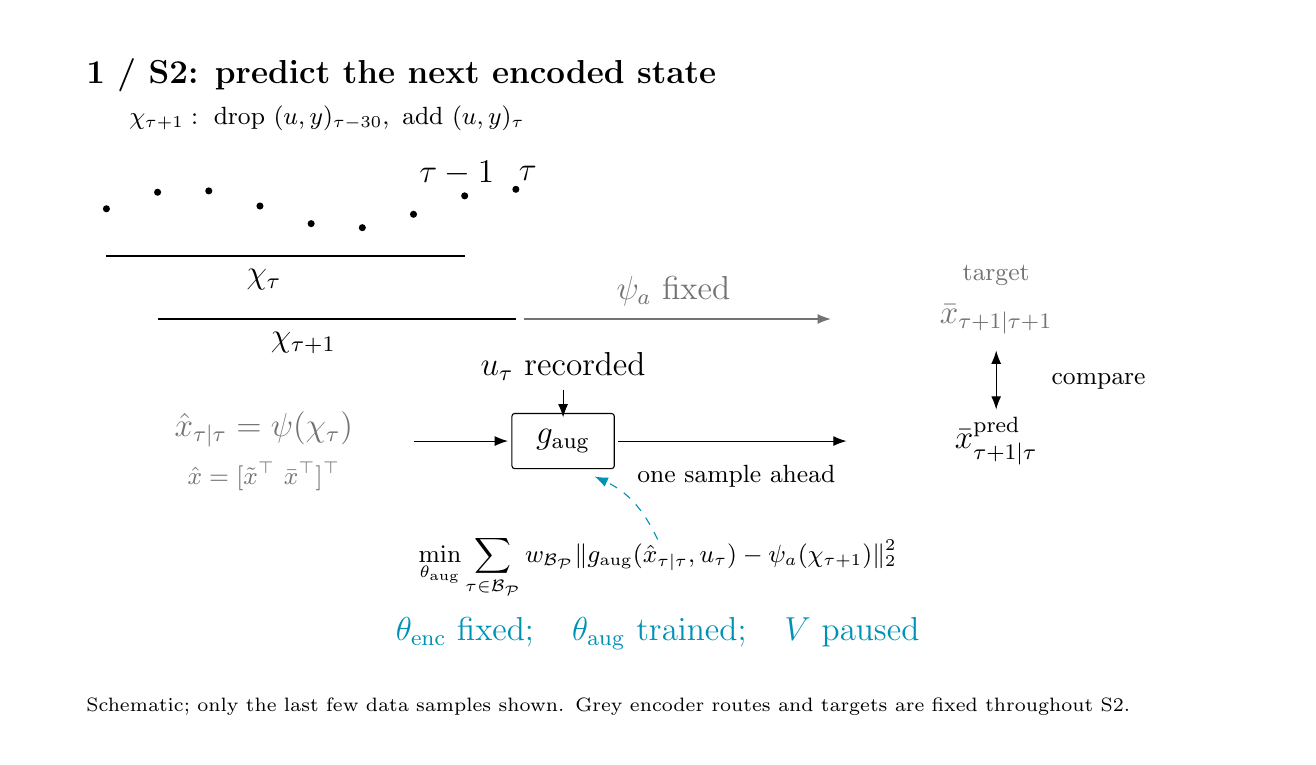
\begin{tikzpicture}\useasboundingbox (0,0) rectangle (16,9);\fill[white] (0,0) rectangle (16,9);\fontsize{12}{14}\selectfont
\node[anchor=west,font=\large\bfseries] at (0.6,8.4) {1 / S2: predict the next encoded state};
\node[anchor=west,font=\scriptsize,text width=14.8cm,align=left] at (0.6,0.38) {Schematic; only the last few data samples shown. Grey encoder routes and targets are fixed throughout S2.};
\fill (1.0,6.700) circle (.045);
\fill (1.65,6.910) circle (.045);
\fill (2.3,6.927) circle (.045);
\fill (2.95,6.735) circle (.045);
\fill (3.6,6.511) circle (.045);
\fill (4.25,6.460) circle (.045);
\fill (4.9,6.630) circle (.045);
\fill (5.55,6.864) circle (.045);
\fill (6.2,6.947) circle (.045);
\node[] at (5.45,7.15) {$\tau-1$};
\node[] at (6.35,7.15) {$\tau$};
\draw[black] (1,6.1) -- (5.55,6.1);
\node[] at (3,5.8) {$\chi_\tau$};
\draw[black] (1.65,5.3) -- (6.2,5.3);
\node[black] at (3.5,5) {$\chi_{\tau+1}$};
\node[black,font=\small] at (3.8,7.85) {$\chi_{\tau+1}:\ \text{drop }(u,y)_{\tau-30},\ \text{add }(u,y)_\tau$};
\draw[->,black!55] (6.3,5.3) -- (10.2,5.3);
\node[black!55] at (8.2,5.65) {$\psi_a$ fixed};
\node[black!55] at (12.3,5.3) {$\bar x_{\tau+1|\tau+1}$};
\node[font=\small,black!55] at (12.3,5.85) {target};
\node[black!55] at (3,3.9) {$\hat x_{\tau|\tau}=\psi(\chi_\tau)$};
\node[font=\small,black!55] at (3,3.3) {$\hat x=[\tilde x^\top\ \bar x^\top]^\top$};
\node[black] at (6.8,4.7) {$u_\tau$ recorded};
\draw[->,black] (6.8,4.4) -- (6.8,4.05);
\node[blk,black] at (6.8,3.75) {$g_{\rm aug}$};
\draw[->,black] (4.9,3.75) -- (6.1,3.75);
\draw[->,black] (7.5,3.75) -- (10.4,3.75);
\node[black] at (12.3,3.75) {$\bar x_{\tau+1|\tau}^{\rm pred}$};
\node[font=\small,black] at (9,3.3) {one sample ahead};
\draw[<->,black] (12.3,4.15) -- (12.3,4.9);
\node[font=\small,black] at (13.6,4.5) {compare};
\node[black,font=\small] at (8,2.15) {$\displaystyle\min_{\theta_{\rm aug}}\sum_{\tau\in\mathcal B_{\mathcal P}}w_{\mathcal B_{\mathcal P}}\|g_{\rm aug}(\hat x_{\tau|\tau},u_\tau)-\psi_a(\chi_{\tau+1})\|_2^2$};
\node[hl] at (8,1.3) {$\theta_{\rm enc}\ \text{fixed};\quad \theta_{\rm aug}\ \text{trained};\quad V\ \text{paused}$};
\draw[->,hl,dashed] (8,2.5) to[bend right=20] (7.2,3.3);
\end{tikzpicture}
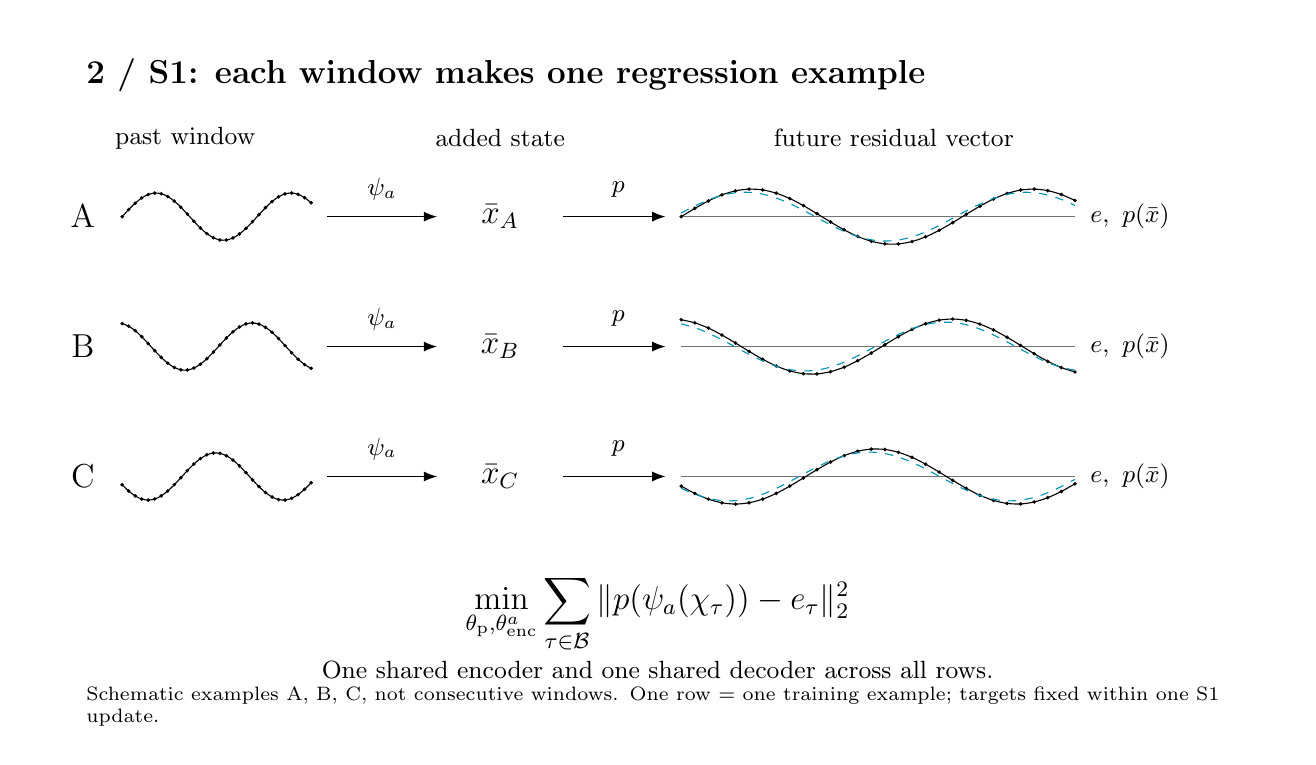
\begin{tikzpicture}\useasboundingbox (0,0) rectangle (16,9);\fill[white] (0,0) rectangle (16,9);\fontsize{12}{14}\selectfont
\node[anchor=west,font=\large\bfseries] at (0.6,8.4) {2 / S1: each window makes one regression example};
\node[anchor=west,font=\scriptsize,text width=14.8cm,align=left] at (0.6,0.38) {Schematic examples A, B, C, not consecutive windows. One row = one training example; targets fixed within one S1 update.};
\node[font=\small] at (2,7.6) {past window};
\node[font=\small] at (6,7.6) {added state};
\node[font=\small] at (11,7.6) {future residual vector};
\node[] at (0.7,6.6) {A};
\draw[] plot[smooth] coordinates {(1.2000,6.6000) (1.2828,6.6896) (1.3655,6.7710) (1.4483,6.8368) (1.5310,6.8810) (1.6138,6.8996) (1.6966,6.8907) (1.7793,6.8554) (1.8621,6.7967) (1.9448,6.7200) (2.0276,6.6324) (2.1103,6.5419) (2.1931,6.4566) (2.2759,6.3844) (2.3586,6.3320) (2.4414,6.3040) (2.5241,6.3030) (2.6069,6.3291) (2.6897,6.3800) (2.7724,6.4509) (2.8552,6.5355) (2.9379,6.6260) (3.0207,6.7141) (3.1034,6.7917) (3.1862,6.8519) (3.2690,6.8891) (3.3517,6.8998) (3.4345,6.8832) (3.5172,6.8408) (3.6000,6.7763)};
\fill[] (1.2000,6.6000) circle (.025);
\fill[] (1.2828,6.6896) circle (.025);
\fill[] (1.3655,6.7710) circle (.025);
\fill[] (1.4483,6.8368) circle (.025);
\fill[] (1.5310,6.8810) circle (.025);
\fill[] (1.6138,6.8996) circle (.025);
\fill[] (1.6966,6.8907) circle (.025);
\fill[] (1.7793,6.8554) circle (.025);
\fill[] (1.8621,6.7967) circle (.025);
\fill[] (1.9448,6.7200) circle (.025);
\fill[] (2.0276,6.6324) circle (.025);
\fill[] (2.1103,6.5419) circle (.025);
\fill[] (2.1931,6.4566) circle (.025);
\fill[] (2.2759,6.3844) circle (.025);
\fill[] (2.3586,6.3320) circle (.025);
\fill[] (2.4414,6.3040) circle (.025);
\fill[] (2.5241,6.3030) circle (.025);
\fill[] (2.6069,6.3291) circle (.025);
\fill[] (2.6897,6.3800) circle (.025);
\fill[] (2.7724,6.4509) circle (.025);
\fill[] (2.8552,6.5355) circle (.025);
\fill[] (2.9379,6.6260) circle (.025);
\fill[] (3.0207,6.7141) circle (.025);
\fill[] (3.1034,6.7917) circle (.025);
\fill[] (3.1862,6.8519) circle (.025);
\fill[] (3.2690,6.8891) circle (.025);
\fill[] (3.3517,6.8998) circle (.025);
\fill[] (3.4345,6.8832) circle (.025);
\fill[] (3.5172,6.8408) circle (.025);
\fill[] (3.6000,6.7763) circle (.025);
\draw[->] (3.8,6.6) -- (5.2,6.6);
\node[font=\small] at (4.5,6.949999999999999) {$\psi_a$};
\node[] at (6,6.6) {$\bar x_{A}$};
\draw[->] (6.8,6.6) -- (8.1,6.6);
\node[font=\small] at (7.5,6.949999999999999) {$p$};
\draw[black!55] (8.3,6.6) -- (13.3,6.6);
\draw[] plot[smooth] coordinates {(8.3000,6.6000) (8.4724,6.7045) (8.6448,6.7995) (8.8172,6.8763) (8.9897,6.9279) (9.1621,6.9495) (9.3345,6.9392) (9.5069,6.8979) (9.6793,6.8295) (9.8517,6.7400) (10.0241,6.6378) (10.1966,6.5322) (10.3690,6.4327) (10.5414,6.3485) (10.7138,6.2873) (10.8862,6.2546) (11.0586,6.2535) (11.2310,6.2840) (11.4034,6.3433) (11.5759,6.4261) (11.7483,6.5248) (11.9207,6.6303) (12.0931,6.7331) (12.2655,6.8237) (12.4379,6.8939) (12.6103,6.9372) (12.7828,6.9498) (12.9552,6.9304) (13.1276,6.8809) (13.3000,6.8057)};
\fill[] (8.3000,6.6000) circle (.025);
\fill[] (8.4724,6.7045) circle (.025);
\fill[] (8.6448,6.7995) circle (.025);
\fill[] (8.8172,6.8763) circle (.025);
\fill[] (8.9897,6.9279) circle (.025);
\fill[] (9.1621,6.9495) circle (.025);
\fill[] (9.3345,6.9392) circle (.025);
\fill[] (9.5069,6.8979) circle (.025);
\fill[] (9.6793,6.8295) circle (.025);
\fill[] (9.8517,6.7400) circle (.025);
\fill[] (10.0241,6.6378) circle (.025);
\fill[] (10.1966,6.5322) circle (.025);
\fill[] (10.3690,6.4327) circle (.025);
\fill[] (10.5414,6.3485) circle (.025);
\fill[] (10.7138,6.2873) circle (.025);
\fill[] (10.8862,6.2546) circle (.025);
\fill[] (11.0586,6.2535) circle (.025);
\fill[] (11.2310,6.2840) circle (.025);
\fill[] (11.4034,6.3433) circle (.025);
\fill[] (11.5759,6.4261) circle (.025);
\fill[] (11.7483,6.5248) circle (.025);
\fill[] (11.9207,6.6303) circle (.025);
\fill[] (12.0931,6.7331) circle (.025);
\fill[] (12.2655,6.8237) circle (.025);
\fill[] (12.4379,6.8939) circle (.025);
\fill[] (12.6103,6.9372) circle (.025);
\fill[] (12.7828,6.9498) circle (.025);
\fill[] (12.9552,6.9304) circle (.025);
\fill[] (13.1276,6.8809) circle (.025);
\fill[] (13.3000,6.8057) circle (.025);
\draw[dashed,hl] plot[smooth] coordinates {(8.3000,6.6463) (8.4724,6.7358) (8.6448,6.8128) (8.8172,6.8704) (8.9897,6.9034) (9.1621,6.9086) (9.3345,6.8856) (9.5069,6.8366) (9.6793,6.7660) (9.8517,6.6802) (10.0241,6.5871) (10.1966,6.4952) (10.3690,6.4128) (10.5414,6.3475) (10.7138,6.3053) (10.8862,6.2900) (11.0586,6.3030) (11.2310,6.3431) (11.4034,6.4067) (11.5759,6.4879) (11.7483,6.5794) (11.9207,6.6727) (12.0931,6.7594) (12.2655,6.8315) (12.4379,6.8825) (12.6103,6.9077) (12.7828,6.9049) (12.9552,6.8741) (13.1276,6.8184) (13.3000,6.7427)};
\node[font=\small] at (14,6.6) {$e,\ p(\bar x)$};
\node[] at (0.7,4.949999999999999) {B};
\draw[] plot[smooth] coordinates {(1.2000,5.2422) (1.2828,5.2085) (1.3655,5.1512) (1.4483,5.0755) (1.5310,4.9884) (1.6138,4.8978) (1.6966,4.8119) (1.7793,4.7387) (1.8621,4.6847) (1.9448,4.6550) (2.0276,4.6522) (2.1103,4.6766) (2.1931,4.7260) (2.2759,4.7958) (2.3586,4.8797) (2.4414,4.9700) (2.5241,5.0585) (2.6069,5.1371) (2.6897,5.1986) (2.7724,5.2374) (2.8552,5.2500) (2.9379,5.2352) (3.0207,5.1943) (3.1034,5.1311) (3.1862,5.0514) (3.2690,4.9625) (3.3517,4.8724) (3.4345,4.7894) (3.5172,4.7210) (3.6000,4.6736)};
\fill[] (1.2000,5.2422) circle (.025);
\fill[] (1.2828,5.2085) circle (.025);
\fill[] (1.3655,5.1512) circle (.025);
\fill[] (1.4483,5.0755) circle (.025);
\fill[] (1.5310,4.9884) circle (.025);
\fill[] (1.6138,4.8978) circle (.025);
\fill[] (1.6966,4.8119) circle (.025);
\fill[] (1.7793,4.7387) circle (.025);
\fill[] (1.8621,4.6847) circle (.025);
\fill[] (1.9448,4.6550) circle (.025);
\fill[] (2.0276,4.6522) circle (.025);
\fill[] (2.1103,4.6766) circle (.025);
\fill[] (2.1931,4.7260) circle (.025);
\fill[] (2.2759,4.7958) circle (.025);
\fill[] (2.3586,4.8797) circle (.025);
\fill[] (2.4414,4.9700) circle (.025);
\fill[] (2.5241,5.0585) circle (.025);
\fill[] (2.6069,5.1371) circle (.025);
\fill[] (2.6897,5.1986) circle (.025);
\fill[] (2.7724,5.2374) circle (.025);
\fill[] (2.8552,5.2500) circle (.025);
\fill[] (2.9379,5.2352) circle (.025);
\fill[] (3.0207,5.1943) circle (.025);
\fill[] (3.1034,5.1311) circle (.025);
\fill[] (3.1862,5.0514) circle (.025);
\fill[] (3.2690,4.9625) circle (.025);
\fill[] (3.3517,4.8724) circle (.025);
\fill[] (3.4345,4.7894) circle (.025);
\fill[] (3.5172,4.7210) circle (.025);
\fill[] (3.6000,4.6736) circle (.025);
\draw[->] (3.8,4.949999999999999) -- (5.2,4.949999999999999);
\node[font=\small] at (4.5,5.299999999999999) {$\psi_a$};
\node[] at (6,4.949999999999999) {$\bar x_{B}$};
\draw[->] (6.8,4.949999999999999) -- (8.1,4.949999999999999);
\node[font=\small] at (7.5,5.299999999999999) {$p$};
\draw[black!55] (8.3,4.949999999999999) -- (13.3,4.949999999999999);
\draw[] plot[smooth] coordinates {(8.3000,5.2908) (8.4724,5.2515) (8.6448,5.1847) (8.8172,5.0964) (8.9897,4.9948) (9.1621,4.8890) (9.3345,4.7889) (9.5069,4.7034) (9.6793,4.6405) (9.8517,4.6058) (10.0241,4.6026) (10.1966,4.6310) (10.3690,4.6886) (10.5414,4.7701) (10.7138,4.8680) (10.8862,4.9733) (11.0586,5.0766) (11.2310,5.1683) (11.4034,5.2400) (11.5759,5.2853) (11.7483,5.3000) (11.9207,5.2827) (12.0931,5.2350) (12.2655,5.1613) (12.4379,5.0684) (12.6103,4.9646) (12.7828,4.8594) (12.9552,4.7626) (13.1276,4.6829) (13.3000,4.6275)};
\fill[] (8.3000,5.2908) circle (.025);
\fill[] (8.4724,5.2515) circle (.025);
\fill[] (8.6448,5.1847) circle (.025);
\fill[] (8.8172,5.0964) circle (.025);
\fill[] (8.9897,4.9948) circle (.025);
\fill[] (9.1621,4.8890) circle (.025);
\fill[] (9.3345,4.7889) circle (.025);
\fill[] (9.5069,4.7034) circle (.025);
\fill[] (9.6793,4.6405) circle (.025);
\fill[] (9.8517,4.6058) circle (.025);
\fill[] (10.0241,4.6026) circle (.025);
\fill[] (10.1966,4.6310) circle (.025);
\fill[] (10.3690,4.6886) circle (.025);
\fill[] (10.5414,4.7701) circle (.025);
\fill[] (10.7138,4.8680) circle (.025);
\fill[] (10.8862,4.9733) circle (.025);
\fill[] (11.0586,5.0766) circle (.025);
\fill[] (11.2310,5.1683) circle (.025);
\fill[] (11.4034,5.2400) circle (.025);
\fill[] (11.5759,5.2853) circle (.025);
\fill[] (11.7483,5.3000) circle (.025);
\fill[] (11.9207,5.2827) circle (.025);
\fill[] (12.0931,5.2350) circle (.025);
\fill[] (12.2655,5.1613) circle (.025);
\fill[] (12.4379,5.0684) circle (.025);
\fill[] (12.6103,4.9646) circle (.025);
\fill[] (12.7828,4.8594) circle (.025);
\fill[] (12.9552,4.7626) circle (.025);
\fill[] (13.1276,4.6829) circle (.025);
\fill[] (13.3000,4.6275) circle (.025);
\draw[dashed,hl] plot[smooth] coordinates {(8.3000,5.2380) (8.4724,5.1906) (8.6448,5.1212) (8.8172,5.0362) (8.9897,4.9433) (9.1621,4.8510) (9.3345,4.7678) (9.5069,4.7012) (9.6793,4.6573) (9.8517,4.6402) (10.0241,4.6513) (10.1966,4.6897) (10.3690,4.7519) (10.5414,4.8322) (10.7138,4.9232) (10.8862,5.0167) (11.0586,5.1040) (11.2310,5.1774) (11.4034,5.2299) (11.5759,5.2569) (11.7483,5.2559) (11.9207,5.2270) (12.0931,5.1727) (12.2655,5.0982) (12.4379,5.0101) (12.6103,4.9165) (12.7828,4.8259) (12.9552,4.7468) (13.1276,4.6861) (13.3000,4.6496)};
\node[font=\small] at (14,4.949999999999999) {$e,\ p(\bar x)$};
\node[] at (0.7,3.3) {C};
\draw[] plot[smooth] coordinates {(1.2000,3.1948) (1.2828,3.1157) (1.3655,3.0534) (1.4483,3.0136) (1.5310,3.0000) (1.6138,3.0138) (1.6966,3.0537) (1.7793,3.1161) (1.8621,3.1953) (1.9448,3.2840) (2.0276,3.3742) (2.1103,3.4577) (2.1931,3.5267) (2.2759,3.5750) (2.3586,3.5983) (2.4414,3.5943) (2.5241,3.5634) (2.6069,3.5085) (2.6897,3.4345) (2.7724,3.3483) (2.8552,3.2576) (2.9379,3.1708) (3.0207,3.0959) (3.1034,3.0395) (3.1862,3.0070) (3.2690,3.0011) (3.3517,3.0226) (3.4345,3.0694) (3.5172,3.1373) (3.6000,3.2200)};
\fill[] (1.2000,3.1948) circle (.025);
\fill[] (1.2828,3.1157) circle (.025);
\fill[] (1.3655,3.0534) circle (.025);
\fill[] (1.4483,3.0136) circle (.025);
\fill[] (1.5310,3.0000) circle (.025);
\fill[] (1.6138,3.0138) circle (.025);
\fill[] (1.6966,3.0537) circle (.025);
\fill[] (1.7793,3.1161) circle (.025);
\fill[] (1.8621,3.1953) circle (.025);
\fill[] (1.9448,3.2840) circle (.025);
\fill[] (2.0276,3.3742) circle (.025);
\fill[] (2.1103,3.4577) circle (.025);
\fill[] (2.1931,3.5267) circle (.025);
\fill[] (2.2759,3.5750) circle (.025);
\fill[] (2.3586,3.5983) circle (.025);
\fill[] (2.4414,3.5943) circle (.025);
\fill[] (2.5241,3.5634) circle (.025);
\fill[] (2.6069,3.5085) circle (.025);
\fill[] (2.6897,3.4345) circle (.025);
\fill[] (2.7724,3.3483) circle (.025);
\fill[] (2.8552,3.2576) circle (.025);
\fill[] (2.9379,3.1708) circle (.025);
\fill[] (3.0207,3.0959) circle (.025);
\fill[] (3.1034,3.0395) circle (.025);
\fill[] (3.1862,3.0070) circle (.025);
\fill[] (3.2690,3.0011) circle (.025);
\fill[] (3.3517,3.0226) circle (.025);
\fill[] (3.4345,3.0694) circle (.025);
\fill[] (3.5172,3.1373) circle (.025);
\fill[] (3.6000,3.2200) circle (.025);
\draw[->] (3.8,3.3) -- (5.2,3.3);
\node[font=\small] at (4.5,3.65) {$\psi_a$};
\node[] at (6,3.3) {$\bar x_{C}$};
\draw[->] (6.8,3.3) -- (8.1,3.3);
\node[font=\small] at (7.5,3.65) {$p$};
\draw[black!55] (8.3,3.3) -- (13.3,3.3);
\draw[] plot[smooth] coordinates {(8.3000,3.1772) (8.4724,3.0849) (8.6448,3.0123) (8.8172,2.9659) (8.9897,2.9500) (9.1621,2.9661) (9.3345,3.0126) (9.5069,3.0854) (9.6793,3.1778) (9.8517,3.2814) (10.0241,3.3866) (10.1966,3.4840) (10.3690,3.5645) (10.5414,3.6209) (10.7138,3.6480) (10.8862,3.6433) (11.0586,3.6073) (11.2310,3.5432) (11.4034,3.4569) (11.5759,3.3563) (11.7483,3.2506) (11.9207,3.1493) (12.0931,3.0618) (12.2655,2.9961) (12.4379,2.9581) (12.6103,2.9513) (12.7828,2.9764) (12.9552,3.0310) (13.1276,3.1102) (13.3000,3.2067)};
\fill[] (8.3000,3.1772) circle (.025);
\fill[] (8.4724,3.0849) circle (.025);
\fill[] (8.6448,3.0123) circle (.025);
\fill[] (8.8172,2.9659) circle (.025);
\fill[] (8.9897,2.9500) circle (.025);
\fill[] (9.1621,2.9661) circle (.025);
\fill[] (9.3345,3.0126) circle (.025);
\fill[] (9.5069,3.0854) circle (.025);
\fill[] (9.6793,3.1778) circle (.025);
\fill[] (9.8517,3.2814) circle (.025);
\fill[] (10.0241,3.3866) circle (.025);
\fill[] (10.1966,3.4840) circle (.025);
\fill[] (10.3690,3.5645) circle (.025);
\fill[] (10.5414,3.6209) circle (.025);
\fill[] (10.7138,3.6480) circle (.025);
\fill[] (10.8862,3.6433) circle (.025);
\fill[] (11.0586,3.6073) circle (.025);
\fill[] (11.2310,3.5432) circle (.025);
\fill[] (11.4034,3.4569) circle (.025);
\fill[] (11.5759,3.3563) circle (.025);
\fill[] (11.7483,3.2506) circle (.025);
\fill[] (11.9207,3.1493) circle (.025);
\fill[] (12.0931,3.0618) circle (.025);
\fill[] (12.2655,2.9961) circle (.025);
\fill[] (12.4379,2.9581) circle (.025);
\fill[] (12.6103,2.9513) circle (.025);
\fill[] (12.7828,2.9764) circle (.025);
\fill[] (12.9552,3.0310) circle (.025);
\fill[] (13.1276,3.1102) circle (.025);
\fill[] (13.3000,3.2067) circle (.025);
\draw[dashed,hl] plot[smooth] coordinates {(8.3000,3.1491) (8.4724,3.0751) (8.6448,3.0216) (8.8172,2.9936) (8.9897,2.9935) (9.1621,3.0214) (9.3345,3.0748) (9.5069,3.1487) (9.6793,3.2364) (9.8517,3.3299) (10.0241,3.4207) (10.1966,3.5005) (10.3690,3.5620) (10.5414,3.5995) (10.7138,3.6097) (10.8862,3.5916) (11.0586,3.5469) (11.2310,3.4797) (11.4034,3.3960) (11.5759,3.3036) (11.7483,3.2108) (11.9207,3.1262) (12.0931,3.0575) (12.2655,3.0109) (12.4379,2.9907) (12.6103,2.9987) (12.7828,3.0343) (12.9552,3.0941) (13.1276,3.1727) (13.3000,3.2629)};
\node[font=\small] at (14,3.3) {$e,\ p(\bar x)$};
\node[] at (8,1.55) {$\displaystyle\min_{\theta_{\rm p},\theta^a_{\rm enc}}\sum_{\tau\in\mathcal B}\|p(\psi_a(\chi_\tau))-e_\tau\|_2^2$};
\node[font=\small] at (8,0.85) {One shared encoder and one shared decoder across all rows.};
\end{tikzpicture}
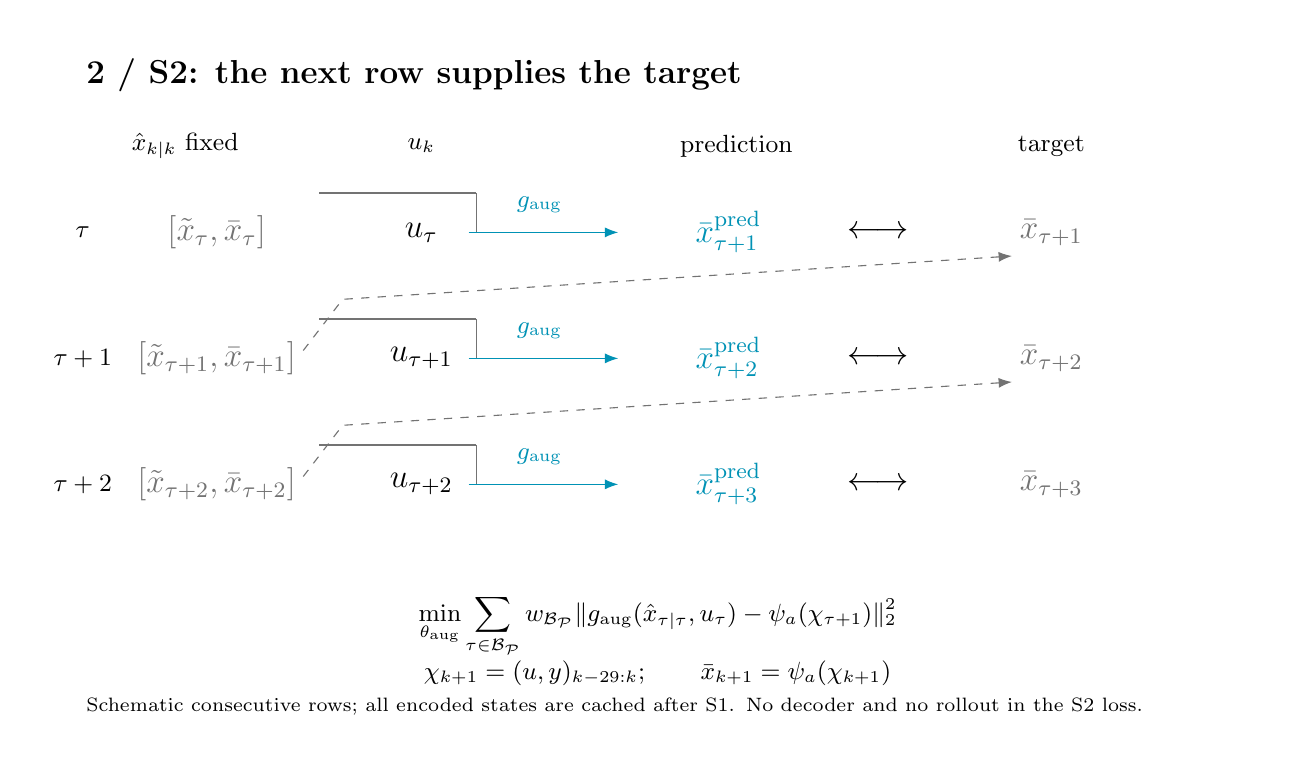
\begin{tikzpicture}\useasboundingbox (0,0) rectangle (16,9);\fill[white] (0,0) rectangle (16,9);\fontsize{12}{14}\selectfont
\node[anchor=west,font=\large\bfseries] at (0.6,8.4) {2 / S2: the next row supplies the target};
\node[anchor=west,font=\scriptsize,text width=14.8cm,align=left] at (0.6,0.38) {Schematic consecutive rows; all encoded states are cached after S1. No decoder and no rollout in the S2 loss.};
\node[font=\small] at (2,7.5) {$\hat x_{k|k}$ fixed};
\node[font=\small] at (5,7.5) {$u_k$};
\node[font=\small] at (9,7.5) {prediction};
\node[font=\small] at (13,7.5) {target};
\node[font=\small] at (0.7,6.4) {$\tau$};
\node[black!55] at (2.4,6.4) {$[\tilde x_{\tau},\bar x_{\tau}]$};
\node[] at (5,6.4) {$u_{\tau}$};
\draw[black!55] (3.7,6.9) -- (5.7,6.9);
\draw[black!55] (5.7,6.9) -- (5.7,6.4);
\draw[->,hl] (5.6,6.4) -- (7.5,6.4);
\node[hl,font=\small] at (6.5,6.75) {$g_{\rm aug}$};
\node[hl] at (8.9,6.4) {$\bar x^{\rm pred}_{\tau+1}$};
\node[] at (10.8,6.4) {$\longleftrightarrow$};
\node[black!55] at (13,6.4) {$\bar x_{\tau+1}$};
\draw[->,black!55,dashed] (3.5,4.9) -- (4,5.550000000000001) -- (12.5,6.1000000000000005);
\node[font=\small] at (0.7,4.800000000000001) {$\tau+1$};
\node[black!55] at (2.4,4.800000000000001) {$[\tilde x_{\tau+1},\bar x_{\tau+1}]$};
\node[] at (5,4.800000000000001) {$u_{\tau+1}$};
\draw[black!55] (3.7,5.300000000000001) -- (5.7,5.300000000000001);
\draw[black!55] (5.7,5.300000000000001) -- (5.7,4.800000000000001);
\draw[->,hl] (5.6,4.800000000000001) -- (7.5,4.800000000000001);
\node[hl,font=\small] at (6.5,5.15) {$g_{\rm aug}$};
\node[hl] at (8.9,4.800000000000001) {$\bar x^{\rm pred}_{\tau+2}$};
\node[] at (10.8,4.800000000000001) {$\longleftrightarrow$};
\node[black!55] at (13,4.800000000000001) {$\bar x_{\tau+2}$};
\draw[->,black!55,dashed] (3.5,3.3000000000000007) -- (4,3.9500000000000006) -- (12.5,4.500000000000001);
\node[font=\small] at (0.7,3.2) {$\tau+2$};
\node[black!55] at (2.4,3.2) {$[\tilde x_{\tau+2},\bar x_{\tau+2}]$};
\node[] at (5,3.2) {$u_{\tau+2}$};
\draw[black!55] (3.7,3.7) -- (5.7,3.7);
\draw[black!55] (5.7,3.7) -- (5.7,3.2);
\draw[->,hl] (5.6,3.2) -- (7.5,3.2);
\node[hl,font=\small] at (6.5,3.5500000000000003) {$g_{\rm aug}$};
\node[hl] at (8.9,3.2) {$\bar x^{\rm pred}_{\tau+3}$};
\node[] at (10.8,3.2) {$\longleftrightarrow$};
\node[black!55] at (13,3.2) {$\bar x_{\tau+3}$};
\node[font=\small] at (8,1.4) {$\displaystyle\min_{\theta_{\rm aug}}\sum_{\tau\in\mathcal B_{\mathcal P}}w_{\mathcal B_{\mathcal P}}\|g_{\rm aug}(\hat x_{\tau|\tau},u_\tau)-\psi_a(\chi_{\tau+1})\|_2^2$};
\node[font=\small] at (8,0.8) {$\chi_{k+1}=(u,y)_{k-29:k};\qquad\bar x_{k+1}=\psi_a(\chi_{k+1})$};
\end{tikzpicture}
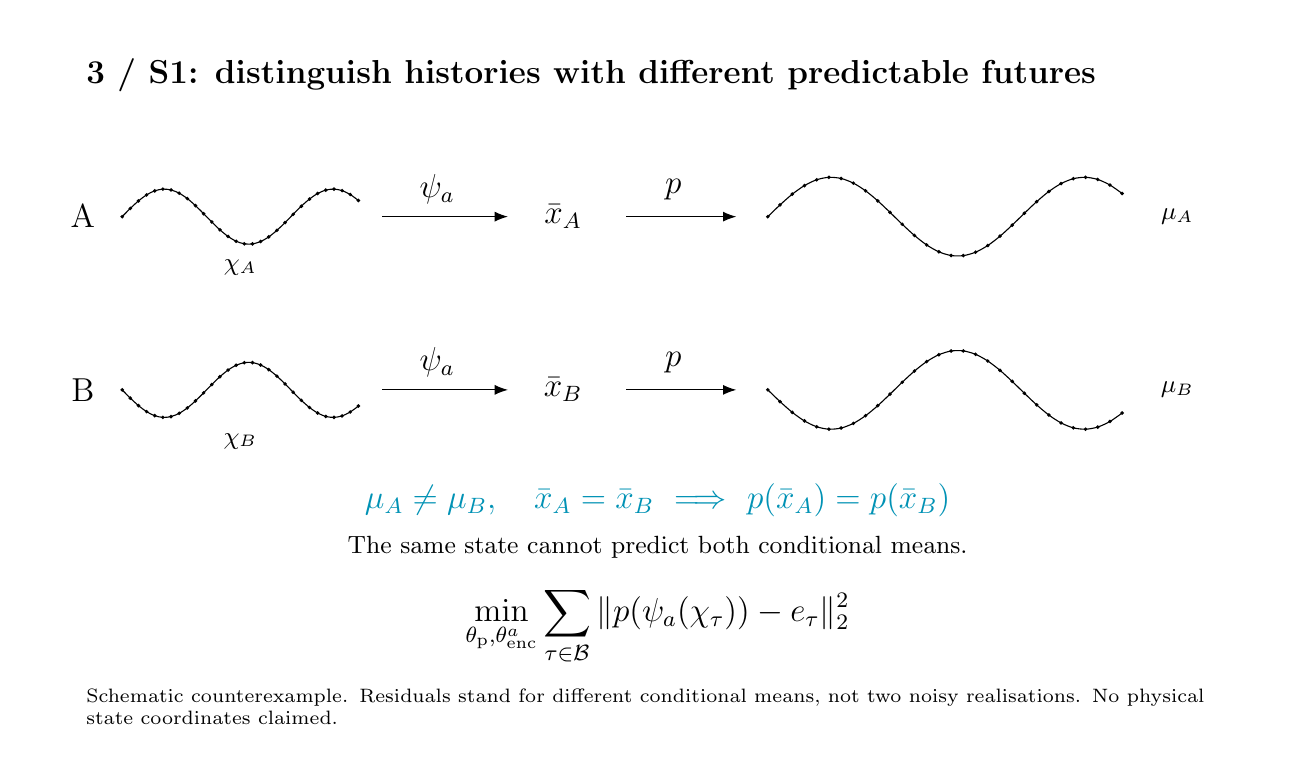
\begin{tikzpicture}\useasboundingbox (0,0) rectangle (16,9);\fill[white] (0,0) rectangle (16,9);\fontsize{12}{14}\selectfont
\node[anchor=west,font=\large\bfseries] at (0.6,8.4) {3 / S1: distinguish histories with different predictable futures};
\node[anchor=west,font=\scriptsize,text width=14.8cm,align=left] at (0.6,0.38) {Schematic counterexample. Residuals stand for different conditional means, not two noisy realisations. No physical state coordinates claimed.};
\node[] at (0.7,6.6) {A};
\draw[] plot[smooth] coordinates {(1.2000,6.6000) (1.3034,6.7045) (1.4069,6.7995) (1.5103,6.8763) (1.6138,6.9279) (1.7172,6.9495) (1.8207,6.9392) (1.9241,6.8979) (2.0276,6.8295) (2.1310,6.7400) (2.2345,6.6378) (2.3379,6.5322) (2.4414,6.4327) (2.5448,6.3485) (2.6483,6.2873) (2.7517,6.2546) (2.8552,6.2535) (2.9586,6.2840) (3.0621,6.3433) (3.1655,6.4261) (3.2690,6.5248) (3.3724,6.6303) (3.4759,6.7331) (3.5793,6.8237) (3.6828,6.8939) (3.7862,6.9372) (3.8897,6.9498) (3.9931,6.9304) (4.0966,6.8809) (4.2000,6.8057)};
\fill[] (1.2000,6.6000) circle (.025);
\fill[] (1.3034,6.7045) circle (.025);
\fill[] (1.4069,6.7995) circle (.025);
\fill[] (1.5103,6.8763) circle (.025);
\fill[] (1.6138,6.9279) circle (.025);
\fill[] (1.7172,6.9495) circle (.025);
\fill[] (1.8207,6.9392) circle (.025);
\fill[] (1.9241,6.8979) circle (.025);
\fill[] (2.0276,6.8295) circle (.025);
\fill[] (2.1310,6.7400) circle (.025);
\fill[] (2.2345,6.6378) circle (.025);
\fill[] (2.3379,6.5322) circle (.025);
\fill[] (2.4414,6.4327) circle (.025);
\fill[] (2.5448,6.3485) circle (.025);
\fill[] (2.6483,6.2873) circle (.025);
\fill[] (2.7517,6.2546) circle (.025);
\fill[] (2.8552,6.2535) circle (.025);
\fill[] (2.9586,6.2840) circle (.025);
\fill[] (3.0621,6.3433) circle (.025);
\fill[] (3.1655,6.4261) circle (.025);
\fill[] (3.2690,6.5248) circle (.025);
\fill[] (3.3724,6.6303) circle (.025);
\fill[] (3.4759,6.7331) circle (.025);
\fill[] (3.5793,6.8237) circle (.025);
\fill[] (3.6828,6.8939) circle (.025);
\fill[] (3.7862,6.9372) circle (.025);
\fill[] (3.8897,6.9498) circle (.025);
\fill[] (3.9931,6.9304) circle (.025);
\fill[] (4.0966,6.8809) circle (.025);
\fill[] (4.2000,6.8057) circle (.025);
\node[font=\small] at (2.7,5.949999999999999) {$\chi_A$};
\draw[->] (4.5,6.6) -- (6.1,6.6);
\node[] at (5.2,6.949999999999999) {$\psi_a$};
\node[] at (6.8,6.6) {$\bar x_A$};
\draw[->] (7.6,6.6) -- (9,6.6);
\node[] at (8.2,6.949999999999999) {$p$};
\draw[] plot[smooth] coordinates {(9.4000,6.6000) (9.5552,6.7493) (9.7103,6.8851) (9.8655,6.9947) (10.0207,7.0684) (10.1759,7.0993) (10.3310,7.0846) (10.4862,7.0256) (10.6414,6.9278) (10.7966,6.8001) (10.9517,6.6541) (11.1069,6.5031) (11.2621,6.3610) (11.4172,6.2407) (11.5724,6.1533) (11.7276,6.1066) (11.8828,6.1050) (12.0379,6.1485) (12.1931,6.2333) (12.3483,6.3516) (12.5034,6.4925) (12.6586,6.6433) (12.8138,6.7901) (12.9690,6.9195) (13.1241,7.0198) (13.2793,7.0818) (13.4345,7.0997) (13.5897,7.0721) (13.7448,7.0013) (13.9000,6.8939)};
\fill[] (9.4000,6.6000) circle (.025);
\fill[] (9.5552,6.7493) circle (.025);
\fill[] (9.7103,6.8851) circle (.025);
\fill[] (9.8655,6.9947) circle (.025);
\fill[] (10.0207,7.0684) circle (.025);
\fill[] (10.1759,7.0993) circle (.025);
\fill[] (10.3310,7.0846) circle (.025);
\fill[] (10.4862,7.0256) circle (.025);
\fill[] (10.6414,6.9278) circle (.025);
\fill[] (10.7966,6.8001) circle (.025);
\fill[] (10.9517,6.6541) circle (.025);
\fill[] (11.1069,6.5031) circle (.025);
\fill[] (11.2621,6.3610) circle (.025);
\fill[] (11.4172,6.2407) circle (.025);
\fill[] (11.5724,6.1533) circle (.025);
\fill[] (11.7276,6.1066) circle (.025);
\fill[] (11.8828,6.1050) circle (.025);
\fill[] (12.0379,6.1485) circle (.025);
\fill[] (12.1931,6.2333) circle (.025);
\fill[] (12.3483,6.3516) circle (.025);
\fill[] (12.5034,6.4925) circle (.025);
\fill[] (12.6586,6.6433) circle (.025);
\fill[] (12.8138,6.7901) circle (.025);
\fill[] (12.9690,6.9195) circle (.025);
\fill[] (13.1241,7.0198) circle (.025);
\fill[] (13.2793,7.0818) circle (.025);
\fill[] (13.4345,7.0997) circle (.025);
\fill[] (13.5897,7.0721) circle (.025);
\fill[] (13.7448,7.0013) circle (.025);
\fill[] (13.9000,6.8939) circle (.025);
\node[font=\small] at (14.6,6.6) {$\mu_A$};
\node[] at (0.7,4.3999999999999995) {B};
\draw[] plot[smooth] coordinates {(1.2000,4.4000) (1.3034,4.2955) (1.4069,4.2005) (1.5103,4.1237) (1.6138,4.0721) (1.7172,4.0505) (1.8207,4.0608) (1.9241,4.1021) (2.0276,4.1705) (2.1310,4.2600) (2.2345,4.3622) (2.3379,4.4678) (2.4414,4.5673) (2.5448,4.6515) (2.6483,4.7127) (2.7517,4.7454) (2.8552,4.7465) (2.9586,4.7160) (3.0621,4.6567) (3.1655,4.5739) (3.2690,4.4752) (3.3724,4.3697) (3.4759,4.2669) (3.5793,4.1763) (3.6828,4.1061) (3.7862,4.0628) (3.8897,4.0502) (3.9931,4.0696) (4.0966,4.1191) (4.2000,4.1943)};
\fill[] (1.2000,4.4000) circle (.025);
\fill[] (1.3034,4.2955) circle (.025);
\fill[] (1.4069,4.2005) circle (.025);
\fill[] (1.5103,4.1237) circle (.025);
\fill[] (1.6138,4.0721) circle (.025);
\fill[] (1.7172,4.0505) circle (.025);
\fill[] (1.8207,4.0608) circle (.025);
\fill[] (1.9241,4.1021) circle (.025);
\fill[] (2.0276,4.1705) circle (.025);
\fill[] (2.1310,4.2600) circle (.025);
\fill[] (2.2345,4.3622) circle (.025);
\fill[] (2.3379,4.4678) circle (.025);
\fill[] (2.4414,4.5673) circle (.025);
\fill[] (2.5448,4.6515) circle (.025);
\fill[] (2.6483,4.7127) circle (.025);
\fill[] (2.7517,4.7454) circle (.025);
\fill[] (2.8552,4.7465) circle (.025);
\fill[] (2.9586,4.7160) circle (.025);
\fill[] (3.0621,4.6567) circle (.025);
\fill[] (3.1655,4.5739) circle (.025);
\fill[] (3.2690,4.4752) circle (.025);
\fill[] (3.3724,4.3697) circle (.025);
\fill[] (3.4759,4.2669) circle (.025);
\fill[] (3.5793,4.1763) circle (.025);
\fill[] (3.6828,4.1061) circle (.025);
\fill[] (3.7862,4.0628) circle (.025);
\fill[] (3.8897,4.0502) circle (.025);
\fill[] (3.9931,4.0696) circle (.025);
\fill[] (4.0966,4.1191) circle (.025);
\fill[] (4.2000,4.1943) circle (.025);
\node[font=\small] at (2.7,3.7499999999999996) {$\chi_B$};
\draw[->] (4.5,4.3999999999999995) -- (6.1,4.3999999999999995);
\node[] at (5.2,4.749999999999999) {$\psi_a$};
\node[] at (6.8,4.3999999999999995) {$\bar x_B$};
\draw[->] (7.6,4.3999999999999995) -- (9,4.3999999999999995);
\node[] at (8.2,4.749999999999999) {$p$};
\draw[] plot[smooth] coordinates {(9.4000,4.4000) (9.5552,4.2507) (9.7103,4.1149) (9.8655,4.0053) (10.0207,3.9316) (10.1759,3.9007) (10.3310,3.9154) (10.4862,3.9744) (10.6414,4.0722) (10.7966,4.1999) (10.9517,4.3459) (11.1069,4.4969) (11.2621,4.6390) (11.4172,4.7593) (11.5724,4.8467) (11.7276,4.8934) (11.8828,4.8950) (12.0379,4.8515) (12.1931,4.7667) (12.3483,4.6484) (12.5034,4.5075) (12.6586,4.3567) (12.8138,4.2099) (12.9690,4.0805) (13.1241,3.9802) (13.2793,3.9182) (13.4345,3.9003) (13.5897,3.9279) (13.7448,3.9987) (13.9000,4.1061)};
\fill[] (9.4000,4.4000) circle (.025);
\fill[] (9.5552,4.2507) circle (.025);
\fill[] (9.7103,4.1149) circle (.025);
\fill[] (9.8655,4.0053) circle (.025);
\fill[] (10.0207,3.9316) circle (.025);
\fill[] (10.1759,3.9007) circle (.025);
\fill[] (10.3310,3.9154) circle (.025);
\fill[] (10.4862,3.9744) circle (.025);
\fill[] (10.6414,4.0722) circle (.025);
\fill[] (10.7966,4.1999) circle (.025);
\fill[] (10.9517,4.3459) circle (.025);
\fill[] (11.1069,4.4969) circle (.025);
\fill[] (11.2621,4.6390) circle (.025);
\fill[] (11.4172,4.7593) circle (.025);
\fill[] (11.5724,4.8467) circle (.025);
\fill[] (11.7276,4.8934) circle (.025);
\fill[] (11.8828,4.8950) circle (.025);
\fill[] (12.0379,4.8515) circle (.025);
\fill[] (12.1931,4.7667) circle (.025);
\fill[] (12.3483,4.6484) circle (.025);
\fill[] (12.5034,4.5075) circle (.025);
\fill[] (12.6586,4.3567) circle (.025);
\fill[] (12.8138,4.2099) circle (.025);
\fill[] (12.9690,4.0805) circle (.025);
\fill[] (13.1241,3.9802) circle (.025);
\fill[] (13.2793,3.9182) circle (.025);
\fill[] (13.4345,3.9003) circle (.025);
\fill[] (13.5897,3.9279) circle (.025);
\fill[] (13.7448,3.9987) circle (.025);
\fill[] (13.9000,4.1061) circle (.025);
\node[font=\small] at (14.6,4.3999999999999995) {$\mu_B$};
\node[hl] at (8,3) {$\mu_A\ne\mu_B,\quad\bar x_A=\bar x_B\ \Longrightarrow\ p(\bar x_A)=p(\bar x_B)$};
\node[font=\small] at (8,2.4) {The same state cannot predict both conditional means.};
\node[] at (8,1.4) {$\displaystyle\min_{\theta_{\rm p},\theta^a_{\rm enc}}\sum_{\tau\in\mathcal B}\|p(\psi_a(\chi_\tau))-e_\tau\|_2^2$};
\end{tikzpicture}
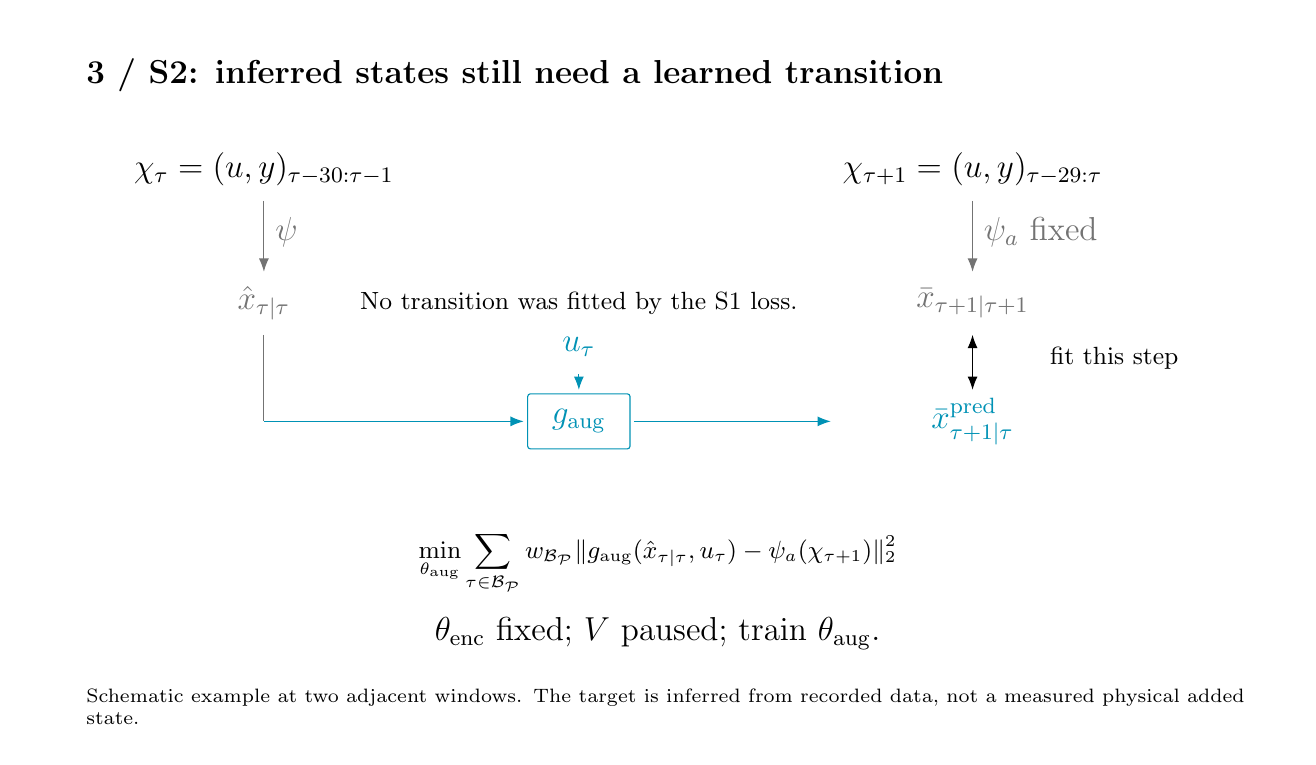
\begin{tikzpicture}\useasboundingbox (0,0) rectangle (16,9);\fill[white] (0,0) rectangle (16,9);\fontsize{12}{14}\selectfont
\node[anchor=west,font=\large\bfseries] at (0.6,8.4) {3 / S2: inferred states still need a learned transition};
\node[anchor=west,font=\scriptsize,text width=14.8cm,align=left] at (0.6,0.38) {Schematic example at two adjacent windows. The target is inferred from recorded data, not a measured physical added state.};
\node[] at (3,7.2) {$\chi_\tau=(u,y)_{\tau-30:\tau-1}$};
\node[] at (12,7.2) {$\chi_{\tau+1}=(u,y)_{\tau-29:\tau}$};
\draw[->,black!55] (3,6.8) -- (3,5.9);
\node[black!55,anchor=west] at (3,6.4) {$\psi$};
\draw[->,black!55] (12,6.8) -- (12,5.9);
\node[black!55,anchor=west] at (12,6.4) {$\psi_a$ fixed};
\node[black!55] at (3,5.5) {$\hat x_{\tau|\tau}$};
\node[black!55] at (12,5.5) {$\bar x_{\tau+1|\tau+1}$};
\node[font=\small] at (7,5.5) {No transition was fitted by the S1 loss.};
\draw[black!55] (3,5.1) -- (3,4);
\draw[->,hl] (3,4) -- (6.3,4);
\node[blk,hl] at (7,4) {$g_{\rm aug}$};
\node[hl] at (7,4.95) {$u_\tau$};
\draw[->,hl] (7,4.6) -- (7,4.4);
\draw[->,hl] (7.7,4) -- (10.2,4);
\node[hl] at (12,4) {$\bar x_{\tau+1|\tau}^{\rm pred}$};
\draw[<->] (12,4.4) -- (12,5.1);
\node[font=\small] at (13.8,4.8) {fit this step};
\node[font=\small] at (8,2.2) {$\displaystyle\min_{\theta_{\rm aug}}\sum_{\tau\in\mathcal B_{\mathcal P}}w_{\mathcal B_{\mathcal P}}\|g_{\rm aug}(\hat x_{\tau|\tau},u_\tau)-\psi_a(\chi_{\tau+1})\|_2^2$};
\node[] at (8,1.3) {$\theta_{\rm enc}$ fixed; $V$ paused; train $\theta_{\rm aug}$.};
\end{tikzpicture}
\end{document}